
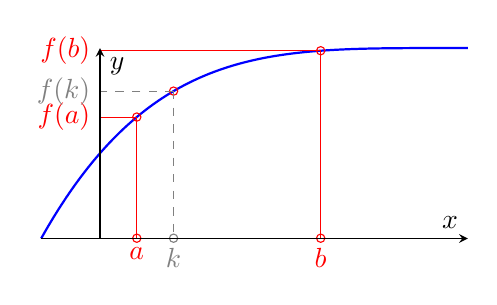
\begin{tikzpicture}
    \begin{axis}[
        axis lines = middle,
        axis on top,
        clip = false,
        xlabel = $x$,
        ylabel = {$y$},
        xtick = \empty,
        ytick = \empty,
        width=7cm,
        height=4cm
    ]
    
    
    \addplot[domain=-0.08:0.5, samples=100, color=blue, thick]{-(x-0.5)^4 + 3}; % Change this function as per your requirement
    
    % Defining the main coordinates
    \coordinate (A) at (axis cs:0.05,2.95899);
    \coordinate (K) at (axis cs:0.1,2.9744);
    \coordinate (B) at (axis cs:0.3, 2.9984);
    \coordinate (Ax) at (axis cs:0.05,2.887);
    \coordinate (Kx) at (axis cs:0.1,2.887);
    \coordinate (Bx) at (axis cs:0.3,2.887);
    \coordinate (Ay) at (axis cs:0,2.95899);
    \coordinate (By) at (axis cs:0, 2.9984);
    \coordinate (Ky) at (axis cs:0,2.9744);
    
    \draw[red] (A) circle [radius=1.5pt];
    \draw[red] (B) circle [radius=1.5pt];
    \draw[red] (K) circle [radius=1.5pt];
    
    \draw[red, solid] (A) -- (Ax)   node[at end, below] {$a$};
    \draw[red, solid] (B) -- (Bx)   node[at end, below] {$b$};
    \draw[gray, dashed] (K) -- (Kx) node[at end, below] {$k$};
    
    \draw[red, solid] (A) -- (Ay) node[at end, left] {$f(a)$};
    \draw[red, solid] (B) -- (By) node[at end, left] {$f(b)$};
    \draw[gray, dashed] (K) -- (Ky) node[at end, left] {$f(k)$};
    
    \draw[red] (Ax) circle [radius=1.5pt];
    \draw[red] (Bx) circle [radius=1.5pt];
    \draw[gray] (Kx) circle [radius=1.5pt];
    
    \end{axis}
    \end{tikzpicture}
    